
\chapter{实验结果}
\label{cha:experiment}

在本章中,我们完整地展示了 F2000 模式分量的代码生成、编译、运行、数据分析等步骤。

\section{配置文件}

\usetikzlibrary{trees}
\tikzstyle{every node}=[draw=black,thick,anchor=west]
\tikzstyle{selected}=[draw=red,fill=red!30]
\tikzstyle{optional}=[dashed,fill=gray!50]

\begin{figure}[H]
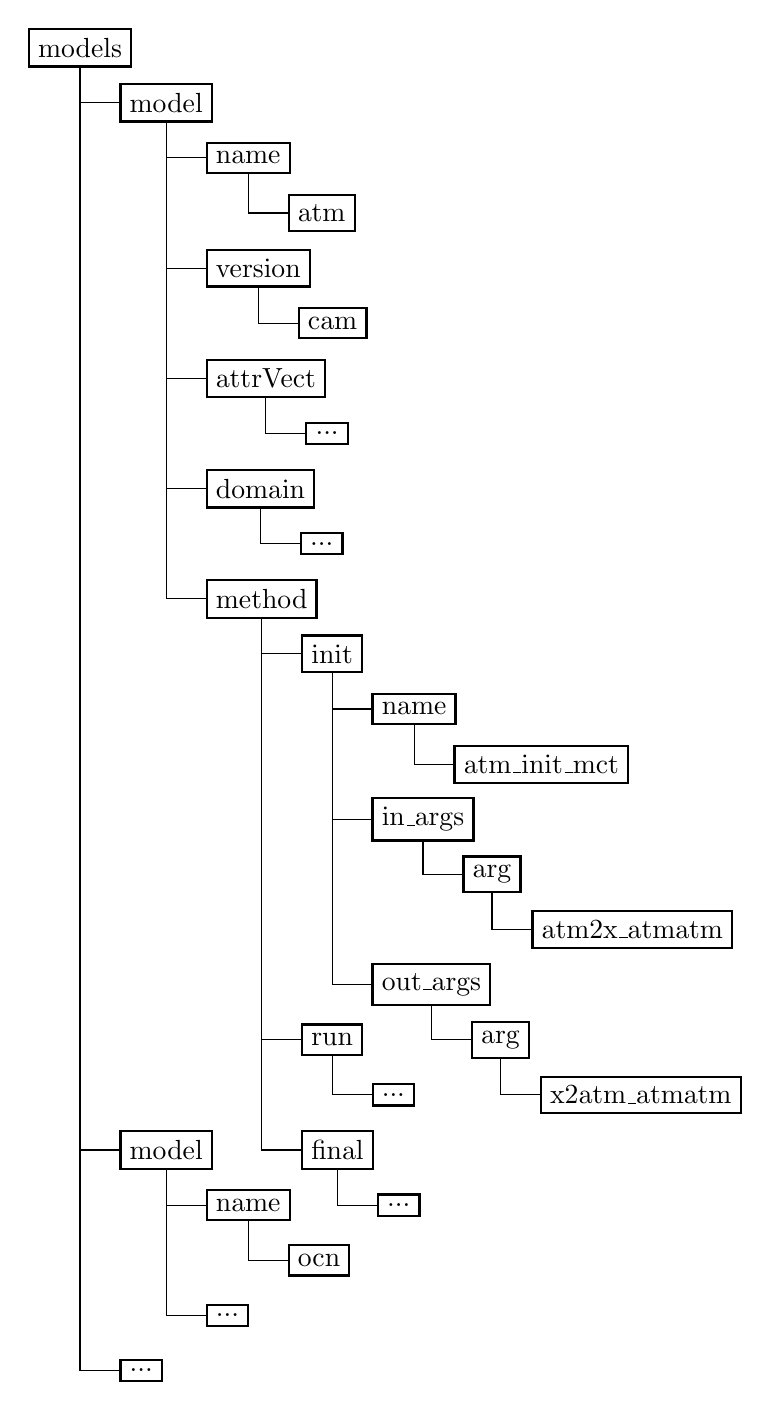
\begin{tikzpicture}[%
  grow via three points={one child at (0.5,-0.7) and
  two children at (0.5,-0.7) and (0.5,-1.4)},
  edge from parent path={(\tikzparentnode.south) |- (\tikzchildnode.west)}]
  \node{models}
  child { node {model}
    child { node {name}
      child {node {atm}}
    }
    child [missing] {}
    child { node {version}
      child {node {cam}}
    }
    child [missing] {}
    child { node {attrVect}
      child {node {...}}
    }
    child [missing] {}    
    child { node {domain}
      child {node {...}}
    }
    child [missing] {}    
    child { node {method}
      child {node {init}
        child { node {name}
        	child { node {atm\_init\_mct}}
        }
        child [missing] {}
        child { node {in\_args}
          child { node {arg}
            child { node {atm2x\_atmatm}}
          }
        }
        child [missing] {}
        child [missing] {}
        child { node {out\_args}
          child { node {arg}
            child { node {x2atm\_atmatm}}
          }
        }
        child [missing] {}
        child [missing] {}
      }
      child [missing] {}
      child [missing] {}
      child [missing] {}
      child [missing] {}
      child [missing] {}
      child [missing] {}
      child {node {run}
        child { node {...} }
      }
      child [missing] {}    
      child {node {final}
        child { node {...} }
      }
      child [missing] {}    
    }
  }
  child [missing] {}    
  child [missing] {}    
  child [missing] {}    
  child [missing] {}    
  child [missing] {}    
  child [missing] {}    
  child [missing] {}    
  child [missing] {}    
  child [missing] {}    
  child [missing] {}    
  child [missing] {}    
  child [missing] {}    
  child [missing] {}    
  child [missing] {}    
  child [missing] {}    
  child [missing] {}    
  child [missing] {}    
  child [missing] {}    
  child { node {model}
    child { node {name}
      child { node {ocn} }
    }
    child [missing] {}
    child { node {...} }
  }
  child [missing] {}
  child [missing] {}
  child [missing] {}
  child {node {...}};
\end{tikzpicture}
\caption{models.xml 结构示意图}
\end{figure}


\begin{figure}[H]
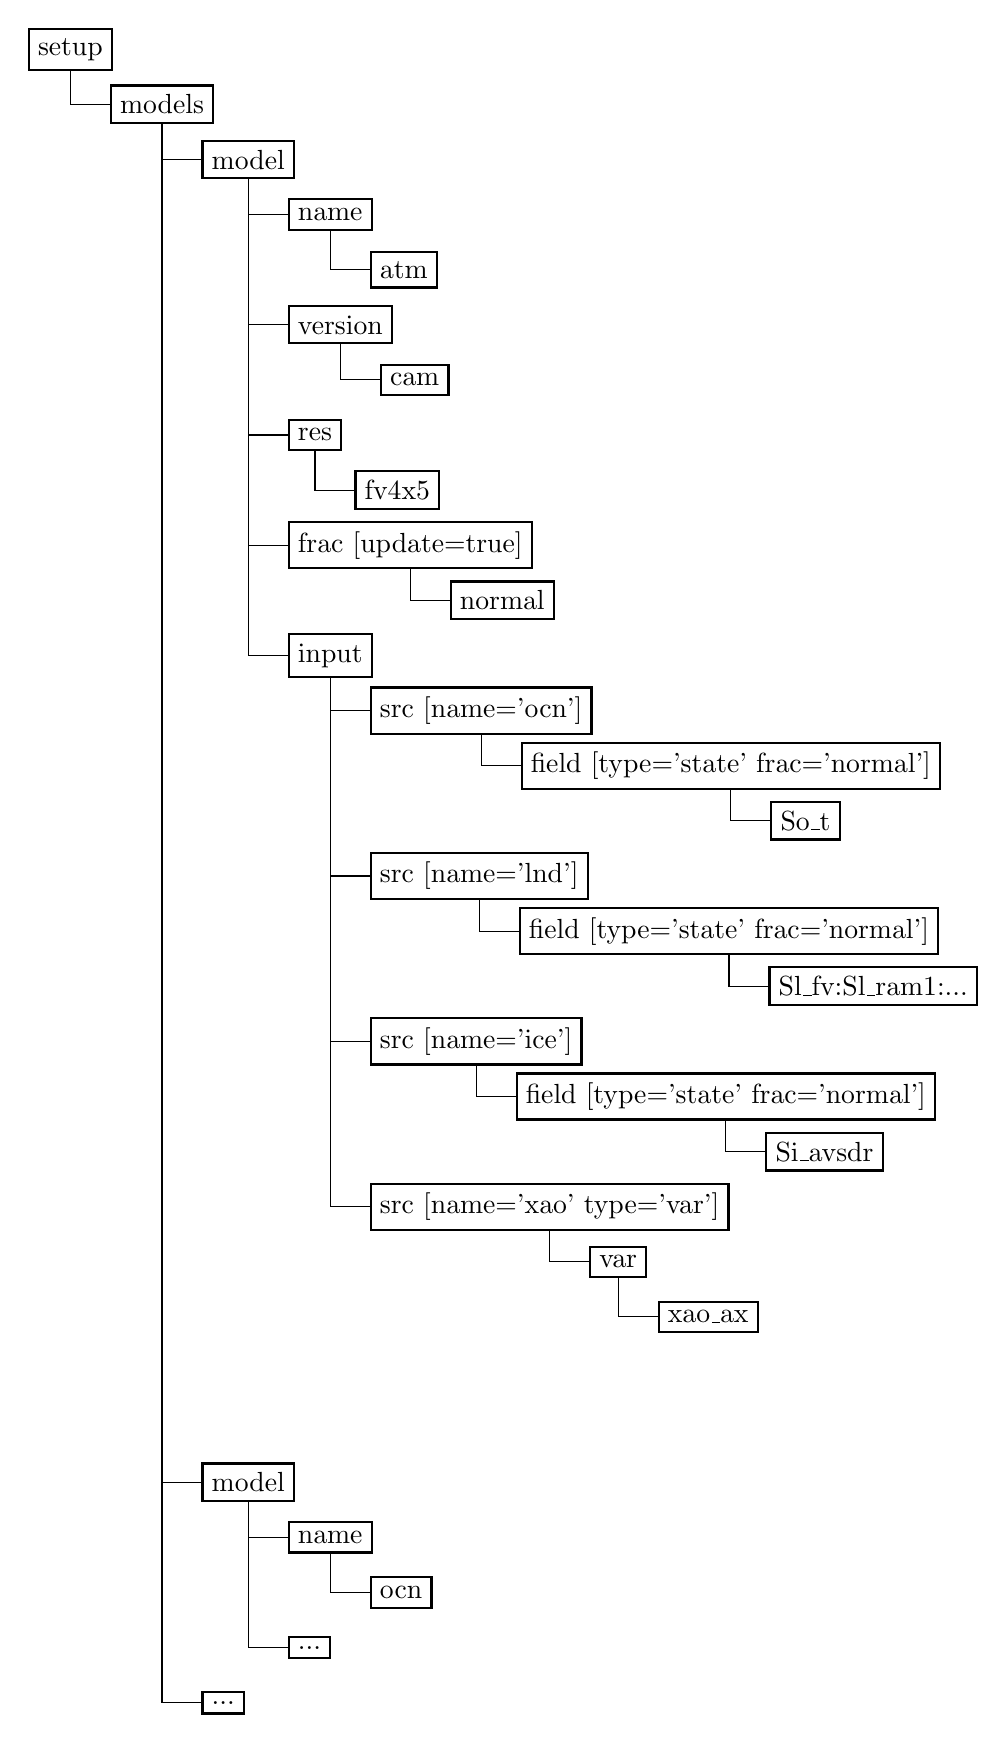
\begin{tikzpicture}[%
  grow via three points={one child at (0.5,-0.7) and
  two children at (0.5,-0.7) and (0.5,-1.4)},
  edge from parent path={(\tikzparentnode.south) |- (\tikzchildnode.west)}]
  \node {setup}
    child { node {models} 
      child { node {model}
        child { node {name}
          child { node {atm} }
        }
        child [missing] {}
        child { node {version}
          child { node {cam} }
        }
        child [missing] {}    		
        child { node {res}
          child { node {fv4x5} }
        }
        child [missing] {}
        child { node {frac [update=true]}
          child { node {normal} }
        }
        child [missing] {}
        child { node {input}
          child { node {src [name='ocn']} 
          	child { node {field [type='state' frac='normal']}
          	  child {node {So\_t}}
          	}
          	child [missing] {}          	
          }
          child [missing] {}
          child [missing] {}
          child { node {src [name='lnd']} 
          	child { node {field [type='state' frac='normal']}
          	  child {node {Sl\_fv:Sl\_ram1:...}}
          	}
          	child [missing] {}          	
          }
          child [missing] {}
          child [missing] {}
          child { node {src [name='ice']} 
          	child { node {field [type='state' frac='normal']}
          	  child {node {Si\_avsdr}}
          	}
          	child [missing] {}          	
          }
          child [missing] {}
          child [missing] {}          
          child { node {src [name='xao' type='var']} 
          	child { node {var}
          	  child {node {xao\_ax}}
          	}
          	child [missing] {}      	
          }
          child [missing] {}
          child [missing] {}        }
        child [missing] {}
      }
      child [missing] {}
      child [missing] {}
      child [missing] {}
      child [missing] {}
      child [missing] {}
      child [missing] {}
      child [missing] {}
      child [missing] {}
      child [missing] {}
      child [missing] {}
      child [missing] {}
      child [missing] {}
      child [missing] {}
      child [missing] {}
      child [missing] {}
      child [missing] {}
      child [missing] {}
      child [missing] {}
      child [missing] {}
      child [missing] {}
      child [missing] {}
      child [missing] {}
      child [missing] {}
      child { node {model}
        child { node {name}
          child { node {ocn} }
        }
        child [missing] {}
        child { node {...} }
      }
      child [missing] {}
      child [missing] {}
      child [missing] {}
      child { node {...} } 
    };
\end{tikzpicture}
\caption{setup.xml 结构示意图}
\end{figure}

\begin{figure}[H]
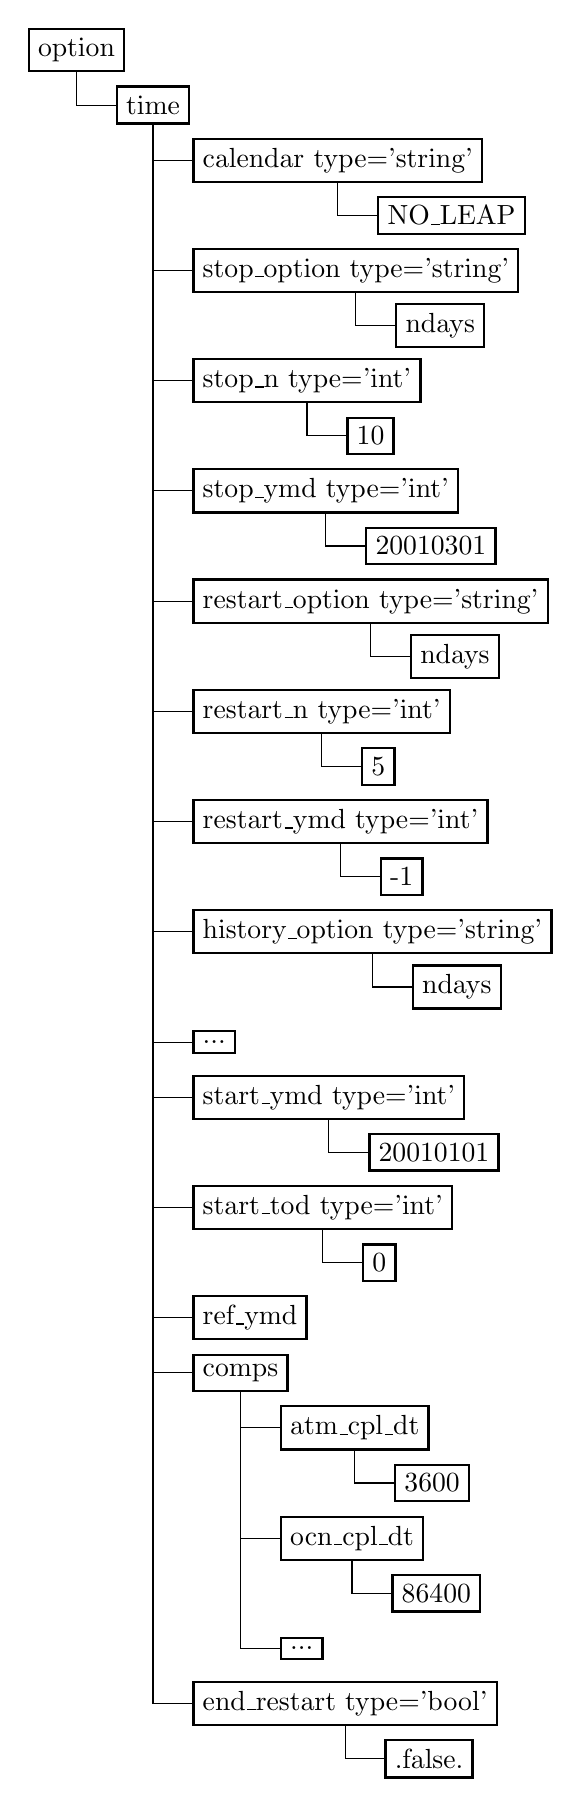
\begin{tikzpicture}[%
  grow via three points={one child at (0.5,-0.7) and
  two children at (0.5,-0.7) and (0.5,-1.4)},
  edge from parent path={(\tikzparentnode.south) |- (\tikzchildnode.west)}]
  \node{option}
  child{ node {time}
    child { node {calendar type='string'}
      child { node {NO\_LEAP} }
    }
    child [missing] {}
    child { node {stop\_option type='string'}
      child {node {ndays}}
    }
    child [missing] {}
    child { node {stop\_n type='int'}
      child {node {10}}
    }
    child [missing] {}
    child { node {stop\_ymd type='int'}
      child {node {20010301}}
    }
    child [missing] {}
    child { node {restart\_option type='string'}
      child {node {ndays}}
    }
    child [missing] {}
    child { node {restart\_n type='int'}
      child {node {5}}
    }
    child [missing] {}
    child { node {restart\_ymd type='int'}
      child {node {-1}}
    }
    child [missing] {}
    child { node {history\_option type='string'}
      child {node {ndays}}
    }
    child [missing] {}
    child { node {...}}
    child { node {start\_ymd type='int'}
      child {node {20010101}}
    }
    child [missing] {}
    child { node {start\_tod type='int'}
      child {node {0}}
    }
    child [missing] {}
    child { node {ref\_ymd} }
    child { node {comps}
      child {node {atm\_cpl\_dt}
        child {node {3600}}
      }
      child [missing] {}
      child {node {ocn\_cpl\_dt}
        child {node {86400}}
      }
      child [missing] {}
      child {node {...} }
    }
    child [missing] {}
    child [missing] {}
    child [missing] {}
    child [missing] {}
    child [missing] {}
    child { node {end\_restart type='bool'}
      child {node {.false.}}
    }
  };
\end{tikzpicture}
\caption{option.xml 结构示意图}
\end{figure}

\begin{figure}[H]
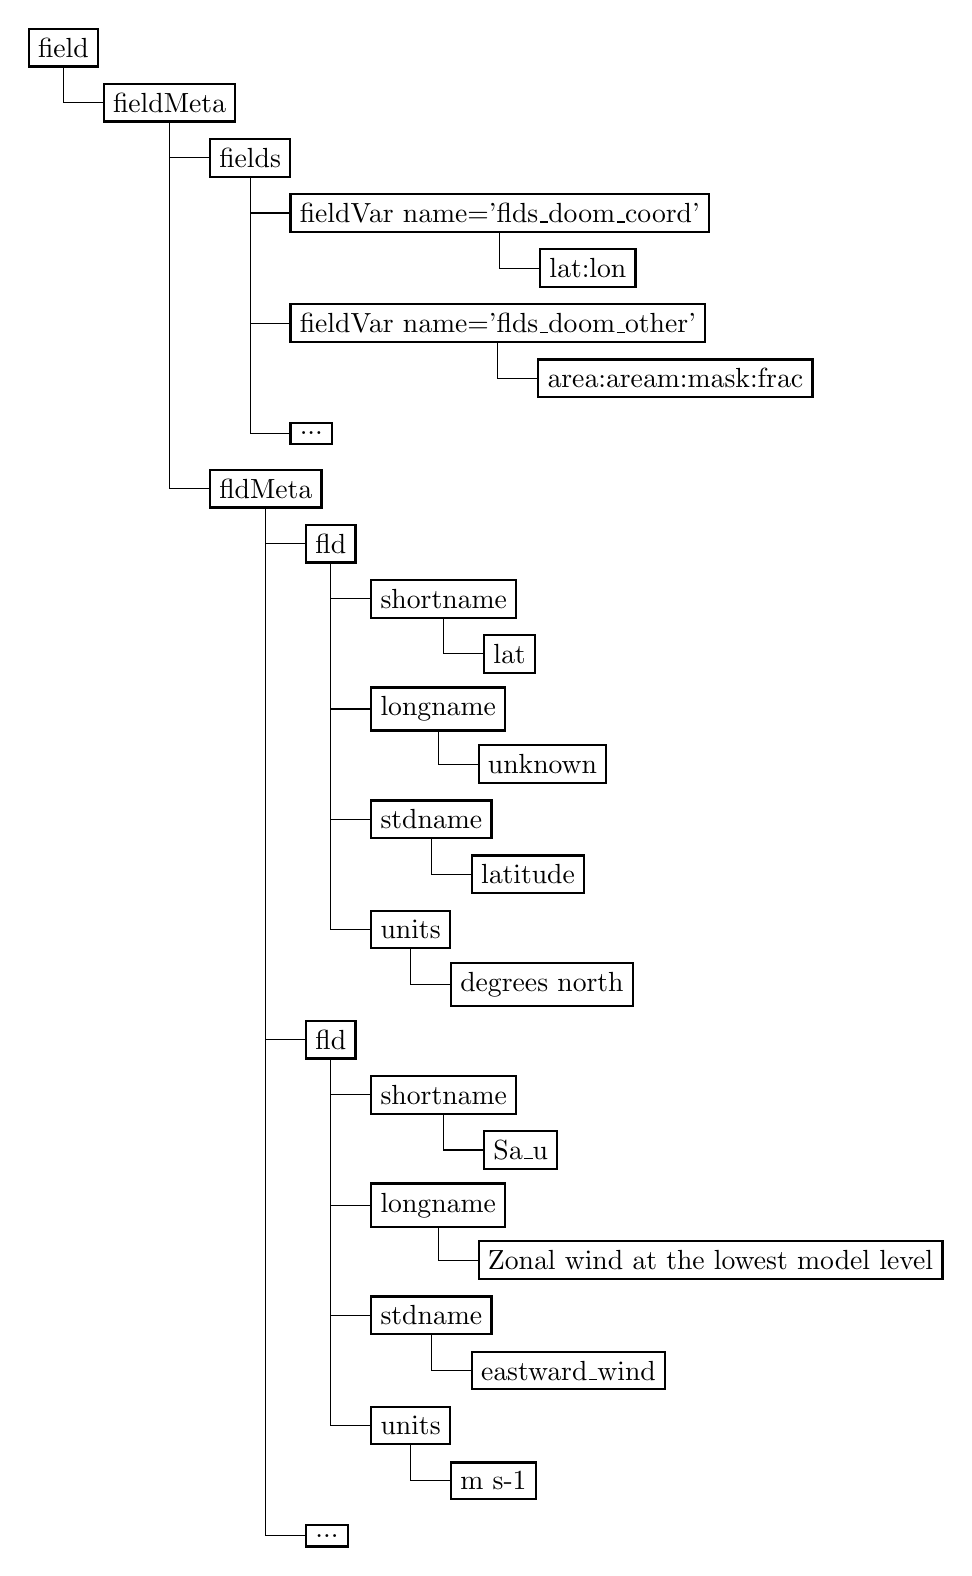
\begin{tikzpicture}[%
  grow via three points={one child at (0.5,-0.7) and
  two children at (0.5,-0.7) and (0.5,-1.4)},
  edge from parent path={(\tikzparentnode.south) |- (\tikzchildnode.west)}]

  \node{field}
  child { node {fieldMeta}
  child { node {fields}
    child { node {fieldVar name='flds\_doom\_coord'}
    	child { node {lat:lon} }
    }
    child [missing] {}
    child { node {fieldVar name='flds\_doom\_other'}
    	child { node {area:aream:mask:frac} }
    }
    child [missing] {}
    child { node {...} }
  }
  child [missing] {}
  child [missing] {}
  child [missing] {}
  child [missing] {}
  child [missing] {}
  child { node {fldMeta}
    child { node {fld}
      child { node {shortname}
        child {node {lat}}
      }
      child [missing] {}
      child { node {longname}
        child {node {unknown}}
      }
      child [missing] {}
      child { node {stdname}
        child {node {latitude}}
      }
      child [missing] {}
      child { node {units}
        child {node {degrees north}}
      }
      child [missing] {}
    }
    child [missing] {}
    child [missing] {}
    child [missing] {}
    child [missing] {}
    child [missing] {}
    child [missing] {}
    child [missing] {}
    child [missing] {}
    child { node {fld}
      child { node {shortname}
        child {node {Sa\_u}}
      }
      child [missing] {}
      child { node {longname}
        child {node {Zonal wind at the lowest model level}}
      }
      child [missing] {}
      child { node {stdname}
        child {node {eastward\_wind}}
      }
      child [missing] {}
      child { node {units}
        child {node {m s-1}}
      }
      child [missing] {}
    }
    child [missing] {}
    child [missing] {}
    child [missing] {}
    child [missing] {}
    child [missing] {}
    child [missing] {}
    child [missing] {}
    child [missing] {}
    child { node {...}}
  }
  };
\end{tikzpicture}
\caption{fields.xml 结构示意图}
\end{figure}

\begin{figure}[H]
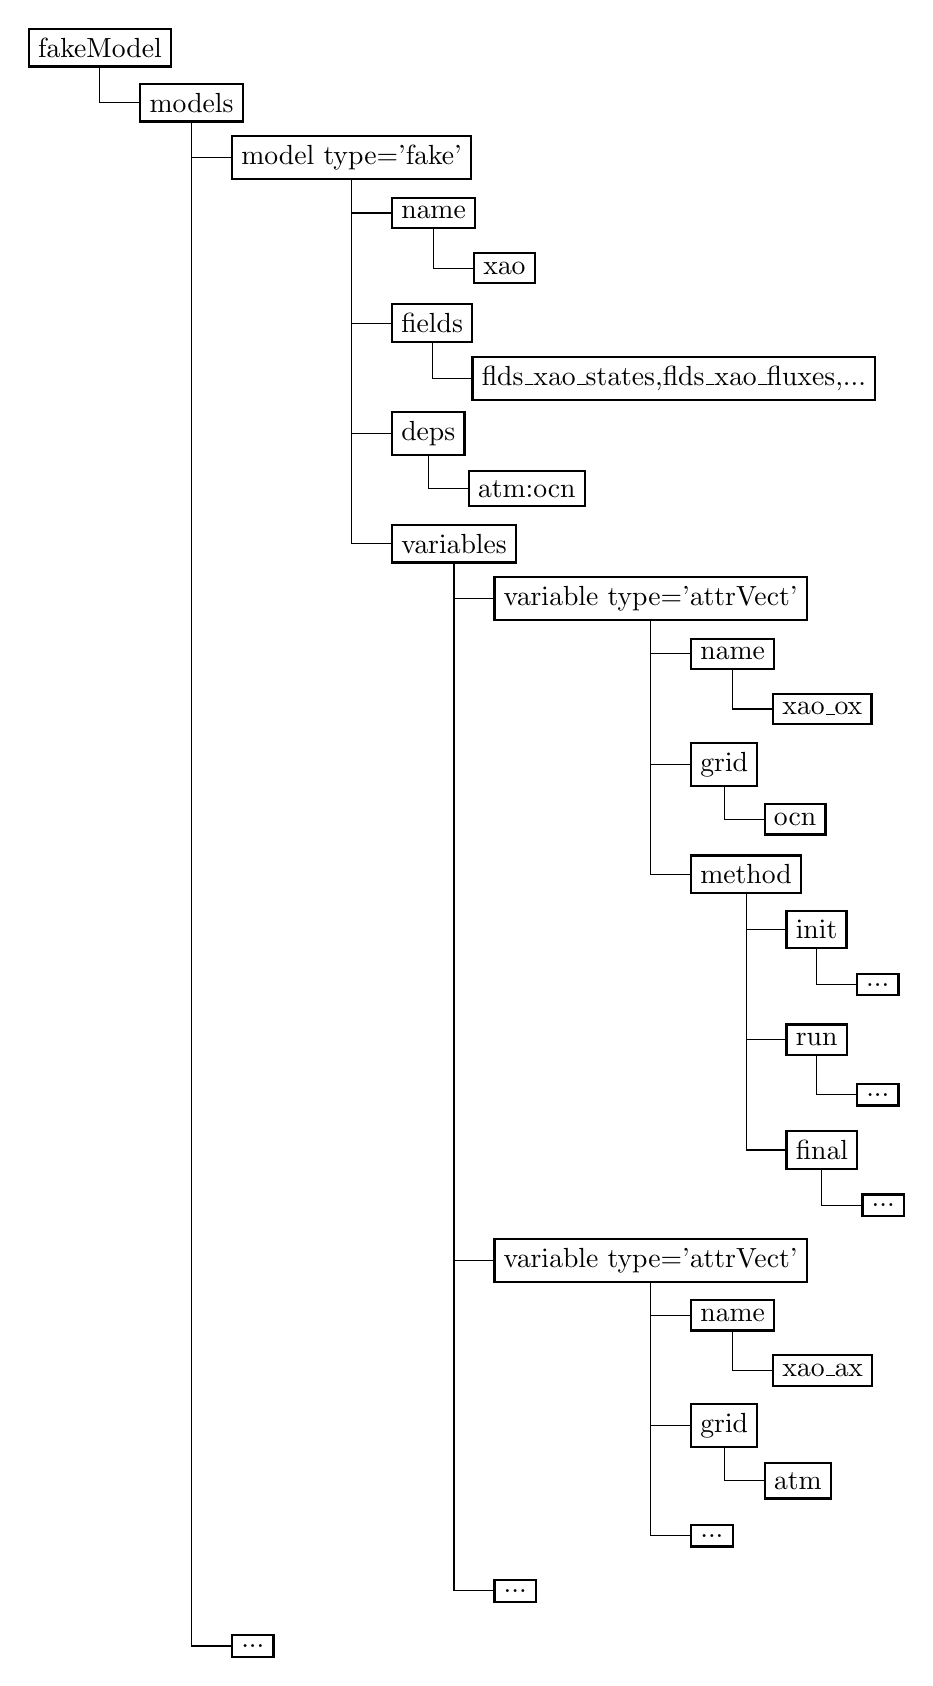
\begin{tikzpicture}[%
  grow via three points={one child at (0.5,-0.7) and
  two children at (0.5,-0.7) and (0.5,-1.4)},
  edge from parent path={(\tikzparentnode.south) |- (\tikzchildnode.west)}]

  \node{fakeModel}
    child { node {models}
    	child { node {model type='fake'}
    		child { node {name}
    			child {node {xao}}
    		}
    		child [missing] {}
    		child { node {fields}
    			child {node {flds\_xao\_states,flds\_xao\_fluxes,...}}
    		}
    		child [missing] {}
    		child { node {deps}
    			child {node {atm:ocn}}
    		}
    		child [missing] {}
    		child { node {variables}
    			child {node {variable type='attrVect'}
    				child { node {name}
    					child {node {xao\_ox}}
    				}
		    		child [missing] {}
    				child { node {grid}
    					child {node {ocn}}
    				}
		    		child [missing] {}
		    		child { node {method}
		    			child { node {init}
		    				child {node {...}}
		    			}
		    			child [missing] {}
		    			child { node {run}
		    				child {node {...}}
		    			}
		    			child [missing] {}
		    			child { node {final}
		    				child {node {...}}
		    			}
		    			child [missing] {}
		    		}
		    		child [missing] {}
		    		child [missing] {}
		    		child [missing] {}
		    		child [missing] {}
		    		child [missing] {}
		    		child [missing] {}
    			}
	    		child [missing] {}
	    		child [missing] {}
	    		child [missing] {}
	    		child [missing] {}
	    		child [missing] {}
	    		child [missing] {}
	    		child [missing] {}
	    		child [missing] {}
	    		child [missing] {}
	    		child [missing] {}
	    		child [missing] {}
    			child {node {variable type='attrVect'}
    				child { node {name}
    					child {node {xao\_ax}}
    				}
		    		child [missing] {}
    				child { node {grid}
    					child {node {atm}}
    				}
		    		child [missing] {}
		    		child { node {...} }
    			}
	    		child [missing] {}
	    		child [missing] {}
	    		child [missing] {}
	    		child [missing] {}
	    		child [missing] {}
    			child {node {...}}
    		}
    	}
   		child [missing] {}
   		child [missing] {}
   		child [missing] {}
   		child [missing] {}
   		child [missing] {}
   		child [missing] {}
   		child [missing] {}
   		child [missing] {}
   		child [missing] {}
   		child [missing] {}
   		child [missing] {}
   		child [missing] {}
   		child [missing] {}
   		child [missing] {}
   		child [missing] {}
   		child [missing] {}
   		child [missing] {}
   		child [missing] {}
   		child [missing] {}
   		child [missing] {}
   		child [missing] {}
   		child [missing] {}
   		child [missing] {}
   		child [missing] {}
   		child [missing] {}
   		child [missing] {}
   		child { node {...} }
    };
\end{tikzpicture}
\caption{fakeModel.xml 结构示意图}
\end{figure}

以上是用户输入的配置文件的主要部分,分别对应 models.xml , setup.xml , option.xml , field.xml ,  fakeModel.xml 五个配置文件。由于篇幅所限部分域用省略号 ... 代替,其余配置文件请参见 github 代码库 \footnote{https://github.com/NeoGeon/BCGen} 。

\section {代码生成}

在用户配置全部录入后,可以通过代码生成模块中的 instCreator 模块进行解析和代码生成。该模块会将解析出的结果以 log 的形式输出到屏幕。若配置正确,应当会产生如下输出:

\begin{lstlisting}
('name', 'atm2x_atmx')
('model', 'atm')
('fraclist', 'afrac:ofrac:lfrac:ifrac')
('init', 'fraction_atm_init')
('update', 'fraction_atm_update')
{'fraclist': 'afrac:ofrac:lfrac:ifrac', 
'init': 'fraction_atm_init', 'update': 
'fraction_atm_update', 'fracs': [{'mapper': 
'mapper_Smatocn2atm', 'model': 'ocn', 'name': 
'ofrac'}, {'mapper': 'mapper_Smatlnd2atm',
'model': 'lnd', 'name': 'lfrac'}, {'mapper':
'mapper_Smatice2atm', 'model': 'ice',
'name': 'ifrac'}]}
...
('name', 'mapper_comp_map')
('arg', 'ocn2x_ocnx')
('arg', 'ocn2x_atmx')
('attrVect', 'lnd2x_lndx')
('field', 'Sl_fv:Sl_ram1:Sl_snowh:Fall_flxdst1:
Fall_flxdst2:Fall_flxdst3:Fall_flxdst4')
...
\end{lstlisting}

\section {内部库预编译}

全部代码生成后会调用 make 工具进行自动内部库编译,若内部库和生成代码格式正确且接口符合,应当会产生如下输出

\begin{lstlisting}
make[1]: Entering directory `/home/hq/git
/protected/BCGen/baseCpl/src/logUtils'
mpif90 -c -I/home/hq/git/protected/BCGen/
baseCpl/include -L/home/hq/git/protected/
BCGen/baseCpl/lib logUtil.F90 
mv *.o /home/hq/git/protected/BCGen/baseCpl/lib
mv *.mod /home/hq/git/protected/BCGen/baseCpl/include
make[1]: Leaving directory 
...
Checking whether input datasets exist locally...
OK -- found depvel_file = /mnt/CESM-data/inputdata/
atm/cam/chem/trop_mozart/dvel/depvel_monthly.nc
OK -- found tracer_cnst_filelist = /mnt/CESM-data/
inputdata/atm/cam/chem/trop_mozart_aero/oxid/
oxid_1.9x2.5_L26_clim_list.c090805.txt
...
\end{lstlisting}

\section {生成实例}

编译后的内部库会与各个模式分量实现的代码一同创建为实验实例,其结构如下图。该实例可以直接编译运行,或对模式分量实现进行嵌入式调试。

\begin{figure}[H]
\begin{tikzpicture}[%
  grow via three points={one child at (0.5,-0.7) and
  two children at (0.5,-0.7) and (0.5,-1.4)},
  edge from parent path={(\tikzparentnode.south) |- (\tikzchildnode.west)}]

  \node{BCGen}
    child { node{BCGen\_inst}
    	child { node {include} 
    		child { node {这里存放内部库和各个模式分量实现的.mod文件} }
    	}
    	child [missing] {}
    	child { node {lib}
    		child { node {这里存放内部库和各个模式分量实现的.o和.a文件} }
    	}
    	child [missing] {}
    	child { node {scripts}
    		child { node {instBuild.sh 自动编译脚本} }
    		child { node {pullDeps.py 自动更新依赖脚本} }
    	}
    	child [missing] {}
    	child [missing] {}
    	child { node {src}
    		child { node {mapper.rc 部分数值文件列表}}
    	}
    	child [missing] {}
    	child { node {models}
    		child { node {cpl}
    			child { node {耦合器主代码,可自动编译为可执行文件} }
    		}
    		child [missing] {}
    		child { node {atm}
    			child { node {大气模式分量实现} }
    		}
    		child [missing] {}
    		child { node {ocn}
    			child { node {海洋模式分量实现} }
    		}
    		child [missing] {}
    		child { node {...} }
    	}
    };
\end{tikzpicture}
\caption{生成实例结构示意图}
\end{figure}

\section {数据分析}

通过 ncl\footnote{http://www.ncl.ucar.edu/Applications/maponly.shtml} 语言对输出的 NetCDF 数据进行作图,可以得出可视化结果。以下为其中一例数据结构:

\begin{figure}[H]
\centering
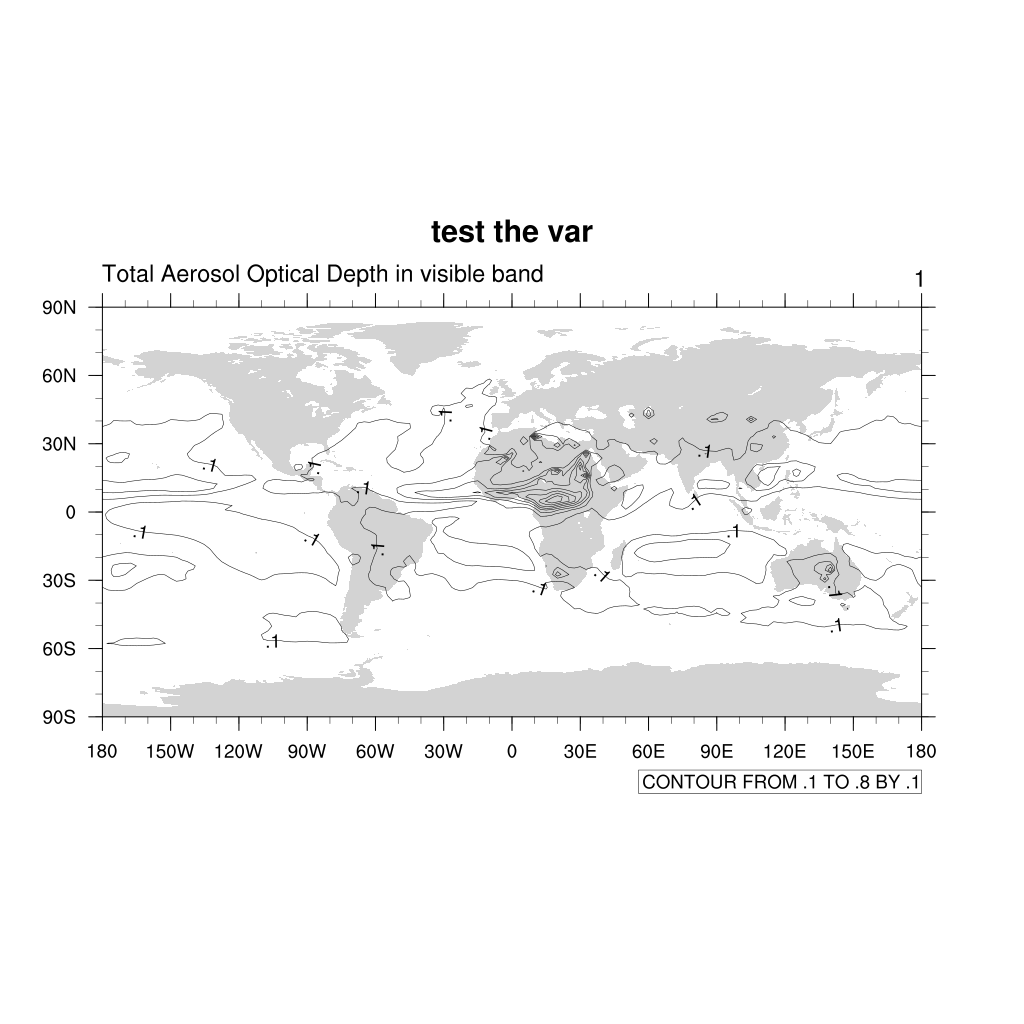
\includegraphics[width=1\textwidth]{../figures/test.png}
\caption{数据分析结果图}
\end{figure}
